\documentclass[11pt]{article}
\usepackage[margin=1in]{geometry}
\usepackage{amsmath,amssymb}
\usepackage{graphicx}
\usepackage{hyperref}
\usepackage{natbib}
\usepackage{booktabs}
\usepackage{enumitem}
\usepackage{float}
\usepackage{setspace}
\usepackage{indentfirst}
\doublespacing

\title{Realized Risk and Uneven Protection Under Geo-Indistinguishability}
\author{Rama Tonpe \\ \texttt{rtonpe2@illinois.edu}}
\date{}

\begin{document}
\maketitle

\begin{abstract}
Formal privacy mechanisms bound how much a data release can reveal regardless of what an attacker already knows, but they say little about the risk a particular release actually carries. This is a gap at the center of the debate over the 2020 Census. This paper examines what drives re-identification under geo-indistinguishability (Andr\'es et al., 2013), a location-privacy mechanism that adds planar Laplace noise to coordinates, and how realized risk compares with its guarantees. Using New York City restaurant inspection records, this paper simulates a noisy release and attacks it with a Bayesian linkage attack whose priors are learned from earlier releases. Protection is systematically non-uniform. A record is exposed when no similar record lies within reach of the noise, and what counts as similar depends on what the attacker knows. Building attributes add little to an attacker who knows only locations, but knowing where restaurants of the same cuisine previously operated raises re-identification from 16\% to 67\% at $\varepsilon = 0.01$. This is almost entirely among restaurants that appeared in earlier releases. As a result, protection varies across boroughs, and which areas are best protected changes with the priors available to the attacker. The mechanism's bounds hold for every record but sit two to three orders of magnitude above realized posterior-to-prior ratios, and linking repeated records degrades privacy far less than the $n\varepsilon$ composition bound implies. These results suggest that publishers choosing $\varepsilon$ should account for local spatial structure and earlier releases rather than rely on worst-case bounds alone.
\end{abstract}

\section{Introduction}

Government agencies routinely publish administrative records with precise geographic coordinates. Location information can reveal patterns of behavior, health conditions, or economic circumstances, which makes these releases particularly sensitive. Common anonymization strategies, such as aggregating records, encoding column values, or omitting identifying fields, may be insufficient when precise coordinates remain. Even coarsened locations, combined with publicly available auxiliary data, can single out specific individuals (de Montjoye et al., 2013). Formal privacy mechanisms add calibrated noise with a provable guarantee, but noise also reduces the data’s usefulness, so every release trades privacy against utility. The U.S. Census Bureau’s adoption of differential privacy for the 2020 Census brought attention to this tradeoff. Critics argued that the accuracy losses would harm social science research and redistricting (Ruggles et al., 2019; Kenny et al., 2021), and questioned whether the re-identification risk the guarantee protects against reflected the risk actually present in the data (Ruggles and Van Riper, 2022).

Geo-indistinguishability (Andr\'es et al., 2013) adds to differential privacy mechanisms by defining a formal privacy guarantee scaled by physical distance. The paper proves that the guarantee is prior-independent. It bounds the attacker's information gain regardless of their auxiliary knowledge (their Theorem 3.1). However, the paper's empirical evaluation is limited to mechanism-level metrics (noise displacement statistics and bandwidth overhead for location-based service queries). It does not evaluate how the mechanism performs when an attacker has access to correlated auxiliary data, when repeated observations of the same location are available (the composition threat described in their Section 3.3), or when the released data will be used for spatial policy analysis rather than individual queries. These questions are vital when trying to holistically assess if a mechanism is suitable for a data release.

This study examines what drives re-identification under the planar Laplace mechanism, how the realized risk compares with its theoretical guarantee, and what this implies for how agencies release geocoded data. It uses NYC restaurant inspection data, with the PLUTO tax lot database as the reference dataset, to evaluate a Bayesian linkage attack whose priors are learned from earlier releases. A linkage attack attempts to match records in an anonymized dataset to their corresponding entries in an auxiliary dataset with known locations. This evaluation covers re-identification rates under eight prior configurations, utility loss for downstream spatial analyses, and posterior-to-prior belief ratios compared against the mechanism's theoretical bounds. The study additionally evaluates a multi-record attack that exploits the CAMIS identifier linking repeated inspections, directly testing the composition guarantee from Section 3.3 of Andr\'es et al.

The NYC restaurant data was a good candidate for this because it is publicly released with unmasked coordinates. Additionally, it links multiple inspections and the coordinates map to an outside dataset (PLUTO). It makes it possible to simulate what a data publisher can see when privatizing sensitive public data. Some results (such as the specific utility metrics) are dataset-specific. However, patterns related to what drives re-identification and utility loss and what priors are informative can be ported to other datasets that may use the Planar Laplace mechanism for their releases. 

The mechanism’s worst-case guarantee greatly overstates the realized privacy loss. The release shifts the attacker’s belief about the true location far less than the theoretical bound allows, with median posterior-to-prior ratios two to three orders of magnitude below it. The most informative auxiliary knowledge was whether a lot had previously hosted a restaurant of the same cuisine. Earlier, unprotected releases could be a source of privacy leaks as well. Most importantly, the protection the mechanism provides is not uniform. Restaurants with similar restaurants nearby, within reach of the noise, are at lower risk than those without, which suggests that the appropriate $\varepsilon$ may vary by region.

\section{Related Work}

The U.S. Census Bureau's adoption of differential privacy for the 2020 Census is the most prominent case of a formal privacy mechanism applied to a public data release, and the debate it produced frames this paper. The Bureau justified the change with an internal experiment in which it reconstructed individual records from published 2010 tabulations and matched them to commercial data. Critics raised two objections. The first concerned utility, since the added noise would reduce the accuracy of census data for social and economic research (Ruggles et al., 2019) and distort the population counts used in redistricting (Kenny et al., 2021). The second concerned the threat itself. Ruggles and Van Riper (2022) argued that the Bureau never compared its match rates against a null model of random guessing, and that most of the reported matches would be expected by chance. Hotz et al. (2022) argue that statistical agencies should weigh privacy protection against data usability explicitly, and boyd and Sarathy (2022) describe how the two sides of the debate relied on different understandings of what the data represent and what privacy requires. Kenny et al. (2023) argue that disclosure avoidance systems should be evaluated by their effects on how the data are actually used. Together, these works point to the need for empirical evaluations of realized risk, with baselines that separate genuine information from chance. The map-only prior and the negative controls in this paper serve that role.

Location is a particularly strong identifier. Sweeney (2000) showed that ZIP code, gender, and date of birth are likely sufficient to uniquely identify 87\% of the U.S. population, and later work formalized anonymity through $k$-anonymity (Sweeney, 2002) and developed statistical estimates of identification risk in microdata (Reiter, 2005). De Montjoye et al. (2013) found that four spatio-temporal points uniquely identify 95\% of individuals in a mobile phone dataset, and that coarsening the data reduces uniqueness only slowly. In a public health setting, Brownstein, Cassa, and Mandl (2006) showed that patient home addresses can be recovered from dot maps printed at the resolution common in medical journals. In each case, re-identification depends on the auxiliary data the attacker brings to the release. The priors in this paper model this auxiliary knowledge explicitly, which makes it possible to measure how much each kind contributes.

Health geographers have long faced the same problem with confidential addresses and developed geographic masks that displace or aggregate point locations before release (Zandbergen, 2014). Kwan, Casas, and Schmitz (2004) showed that larger displacements protect privacy at the cost of distorting the spatial patterns analysts rely on. In this literature, protection is evaluated empirically, most often through spatial $k$-anonymity (the number of potential locations among which the true one is hidden), and the recommended displacement is inversely proportional to local population density (Zandbergen, 2014). No formal guarantee is attached, and no standard for confidentiality protection has emerged. Geo-indistinguishability offers the opposite, a formal guarantee that holds against any attacker but no empirical evaluation of the risk it leaves in practice.

This paper connects these strands. It evaluates a mechanism with a formal guarantee using the kind of realized-risk evaluation the Census debate called for, with baselines and negative controls, auxiliary data learned from earlier releases, and the spatial utility measures used in the geographic masking literature.

\section{Background}

\subsection{Geo-indistinguishability}

Standard differential privacy (Dwork et al., 2006) protects a row in a database by ensuring the output distribution is similar whether that row is included or not. When the ``database'' is a single user's location, this would require the output to be essentially independent of the true location, rendering the service useless. Geo-indistinguishability relaxes this by scaling the privacy guarantee with physical distance.

A mechanism $K$ satisfies $\varepsilon$-geo-indistinguishability if for all locations $x, x'$ and all measurable sets $Z$,
\begin{equation}
K(x)(Z) \leq e^{\varepsilon \cdot d(x,x')} \cdot K(x')(Z)
\end{equation}

The parameter $\varepsilon$ is in inverse distance units and controls the rate at which privacy degrades with distance. The expected displacement is $2/\varepsilon$.

The guarantee is prior-independent. For any prior $\pi$ the attacker holds, the posterior-to-prior ratio is bounded by $e^{\varepsilon \cdot \text{diameter}(N)}$ for any region $N$ (Andr\'es et al., 2013, Theorem 3.1). This is the theoretical ceiling that this paper's empirical evaluation tests against.

\subsection{The planar Laplace mechanism}

The mechanism adds noise from a planar Laplace distribution with density proportional to $e^{-\varepsilon \cdot d}$ at distance $d$ from the true location. Unlike independent 1D Laplace noise on each coordinate, the planar Laplace is radially symmetric, providing uniform privacy in all directions. Sampling uses polar coordinates. The angle $\theta$ is drawn uniformly from $[0, 2\pi)$, the radius $r$ is drawn via the inverse CDF of $C(r) = 1 - (1 + \varepsilon r)e^{-\varepsilon r}$, and $(r \cdot \cos\theta,\; r \cdot \sin\theta)$ is added to the true location.

\subsection{Composition for traces}

Section 3.3 of Andr\'es et al.\ addresses the case where the same location generates $n$ independent noisy observations. Under standard composition, $n$ independent $\varepsilon$-geo-indistinguishable observations degrade to $n\varepsilon$ total privacy loss.

\section{Data and Threat Model}

\subsection{Datasets}

\textbf{NYC DOHMH Restaurant Inspection Results.} Inspection records for restaurants across all five boroughs (NYC Department of Health and Mental Hygiene, 2026). Each record includes a unique restaurant identifier (CAMIS), inspection date, coordinates, borough, cuisine description, violation codes, critical flag, score, and grade. Multiple inspections of the same restaurant share the same CAMIS. Coordinates were projected from WGS84 to NYC State Plane (EPSG:2263, in feet) to ensure Euclidean distances are physically meaningful.

\textbf{NYC PLUTO.} Tax lot records for 857,347 lots across five boroughs (NYC Department of City Planning, 2026), including BBL identifier, coordinates (State Plane), land use code, building class, residential units, floors, year built, building area, and borough. This serves as the attacker's reference dataset.

\subsection{Threat model and data split}

Inspection data was released openly through 2024 with full BBL and address information. Starting in 2025, the publisher anonymizes by adding planar Laplace noise and stripping BBL. The attacker uses historical releases (the training set covers 2020--2024, with 36,960 visits, 20,636 restaurants, of which 36,056 visits join to PLUTO by BBL; because the public dataset retains only recent inspections, over 90\% of training visits date from 2023--2024) to learn priors and attacks the anonymized release (the test set covers inspections from January 1, 2025 to October 9, 2026, 45,052 visits, 25,432 restaurants). The released test data includes noisy coordinates, an updated CAMIS number, inspection date, cuisine description, borough, critical flag, score, and grade. BBL is withheld as its inclusion would make re-identification trivial. The CAMIS is modified as using the same CAMIS as previous releases would provide a direct mapping from CAMIS to BBL (for restaurants that are part of both releases). Moving forward, CAMIS will refer to the pseudonym. Each test record's true location is taken to be the PLUTO coordinate of its lot, and noise is added to that point, so that a correct guess corresponds exactly to the true lot.

PLUTO version 26v2 is used for both training and attack. Only test records whose BBL appears in PLUTO are kept (45,052 of 46,116 geocoded test visits, or 97.7\%); likewise, 36,056 of 36,960 training visits (97.6\%) join to PLUTO. The unmatched BBLs may reflect lots that changed after the inspection or geocoding errors in the inspection data, and this study does not distinguish between the two. BBL for the test dataset is used only during evaluation to verify correctness. It is never provided to the attack algorithm.

\subsection{Attack methodology}

The attack implements the optimal Bayesian strategy from Andr\'es et al.'s theoretical framework. For each noisy observation $z$, the attacker computes
\begin{equation}
\text{score}(x) = \pi(x) \cdot e^{-\varepsilon \cdot d(x, z)}
\end{equation}
for each candidate lot $x$, where $\pi(x)$ is the prior weight and $d(x, z)$ is Euclidean distance. The highest-scoring lot is the guess. Candidates are restricted to lots within a search radius $r$ satisfying $C(r) = 0.99$, derived from the mechanism's CDF, which keeps the attack computationally feasible. This is the MAP estimator, so for a given prior the measured re-identification rate is the highest any attacker holding that prior can achieve. Across attackers, however, it is a lower bound, since an attacker with more informative auxiliary data could do better.

\subsection{Configurations}

A prior assigns each PLUTO lot a weight reflecting how likely the restaurant is to be located there before the attacker sees the noisy point. Lots are divided into groups by some attribute, each group receives the share of restaurant visits that fall in it, and that share is split evenly among the group's lots. Shares are estimated within the training data by predicting where 2024 visits occurred from earlier years; group membership at attack time uses all 2020--2024 records, and zero shares are floored at $10^{-10}$. For example, 56.9\% of 2024 visits took place on lots that had hosted a restaurant before 2024. Under the any-restaurant-history prior, those lots therefore share 56.9\% of the weight and all other lots share the remaining 43.1\%; because far fewer lots have restaurant history, each of them receives a much higher weight. This paper evaluates the following eight priors.
\begin{itemize}[leftmargin=1.5em]
    \item \textbf{Map only.} Every lot is equally likely, so the attacker guesses the lot nearest the noisy point. This is the baseline.
    \item \textbf{Building type.} Groups are PLUTO land-use classes. Captures that restaurants concentrate in a few kinds of buildings (55\% of 2024 visits were in mixed residential and commercial buildings and 37\% in commercial and office buildings).
    \item \textbf{Building type + cuisine.} The same groups as Building Type, with shares estimated separately for each cuisine (Figure~\ref{fig:prior_heatmap}).
    \item \textbf{Any restaurant history.} Two groups, lots that hosted any restaurant in the training period and all other lots.
    \item \textbf{Same-cuisine history.} Two groups defined for each cuisine, lots that hosted a restaurant of that cuisine in the training period and all other lots.
    \item \textbf{Everything.} Lots with same-cuisine history, lots with only other restaurant history, and lots without restaurant history grouped by land-use class, with shares estimated separately for each cuisine.
    \item \textbf{Residential units} and \textbf{year built.} Groups are bins of each attribute, with shares estimated by cuisine. These are negative controls, attributes expected to say little about where a restaurant is, and test whether the evaluation credits gains to any prior.
\end{itemize}
These weights reflect empirical associations, not causal relationships.


\begin{figure}[H]
    \centering
    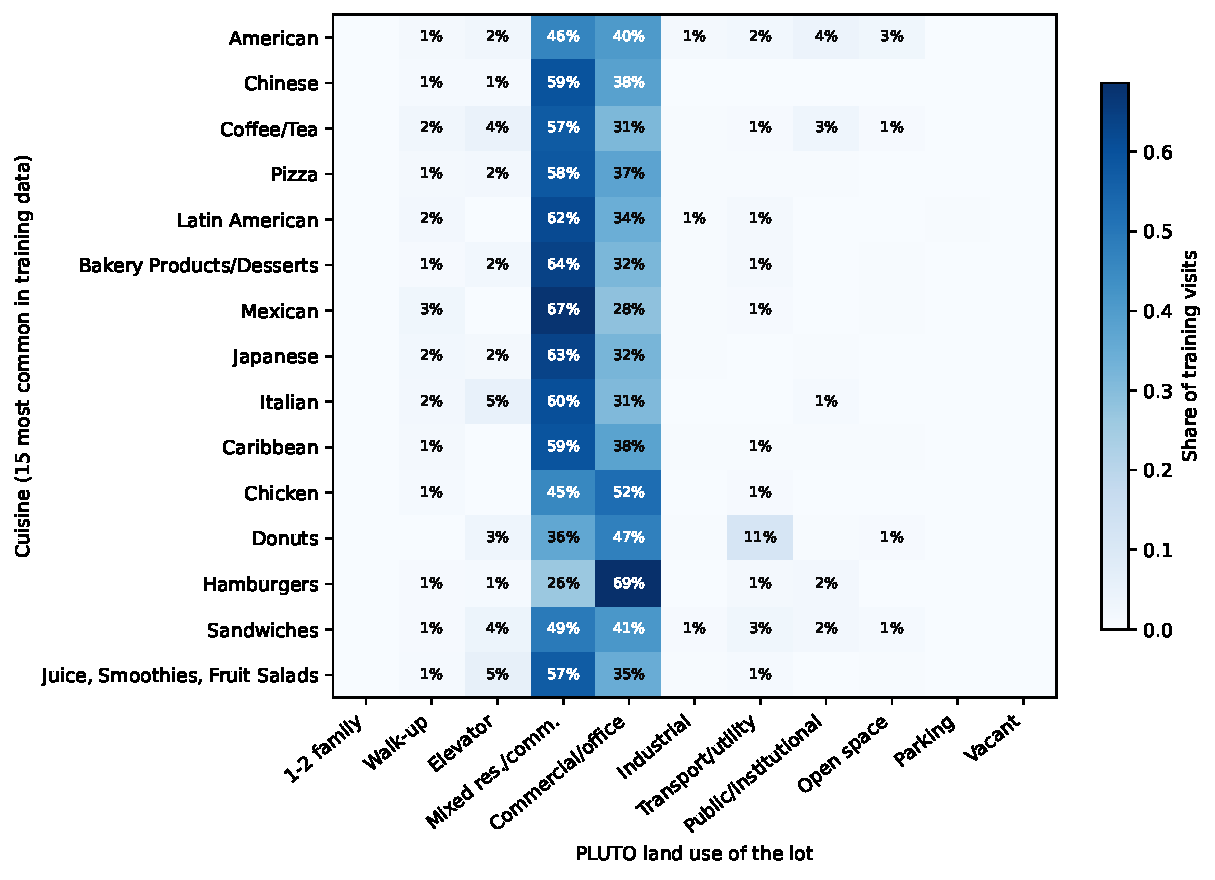
\includegraphics[width=0.8\textwidth]{fig_prior_heatmap.pdf}
    \caption{Share of training visits in each PLUTO land-use class for the 15 most common cuisines (2020--2024).}
    \label{fig:prior_heatmap}
\end{figure}

\subsection{Multi-record attack}

The multi-record attack exploits the CAMIS identifier linking multiple inspections to the same restaurant. When a restaurant is inspected $n$ times and each inspection's coordinates are independently distorted, the attacker observes $n$ noisy points scattered around the same true location. The attack proceeds in four steps. It (1) queries the PLUTO KDTree for all lots within the search radius of each noisy observation, (2) intersects all $n$ candidate sets, (3) computes the joint score
\begin{equation}
\log\text{score}(x) = \log \pi(x) - \varepsilon \cdot \sum_{i=1}^{n} d(x, z_i)
\end{equation}
and (4) selects the highest-scoring candidate. If the intersection is empty, the union is used as fallback.

\section{Evaluation Metrics}

\begin{description}[leftmargin=1.5em, style=nextline]
    \item[Re-identification rate.] The fraction of test records for which the attacker's guess is the true PLUTO lot, verified by BBL match.

    \item[Utility loss.] Distortion of two tract-level statistics, computed over 2020 Census tracts that contain restaurants both before and after noise and weighted by number of records.
    \begin{itemize}[leftmargin=1.5em]
        \item \emph{Inspection score distortion.} RMSE and MAE of mean inspection scores per tract, true vs.\ noisy coordinates.
        \item \emph{Cuisine composition distortion.} Total variation distance (TVD) between each tract's cuisine distribution under true and noisy coordinates, ranging from 0 (identical) to 1 (completely different).
    \end{itemize}

    \item[Posterior-to-prior ratio.] For each record, how much the attacker's belief in the true lot changes after observing the noisy coordinates $z$,
    \begin{equation}
        \frac{P(\text{true lot} \mid z)}{\pi(\text{true lot})},
    \end{equation}
    compared against the bound $e^{\varepsilon D}$ from Theorem 3.1 of Andr\'es et al., where $D$ is the distance from the true lot to the farthest candidate in the search region.
\end{description}

\section{Results}

This paper tests $\varepsilon$ values ranging from 0.001 to 0.05 ft$^{-1}$. Values above about 0.005 fall outside the range explored by Andr\'es et al.\ (corresponding to $\ell = \ln(2)$ to $\ln(6)$ at $r = 200$m, and $\varepsilon \approx 0.005$ ft$^{-1}$ in their mechanism comparison). Higher values are included to characterize the full privacy-utility tradeoff.

\subsection{Single-query re-identification}

Re-identification rises monotonically with $\varepsilon$ under every prior (Figure~\ref{fig:single_query}, left). Under the map-only baseline, the attacker identifies 0.6\% of records at $\varepsilon = 0.001$, 15.9\% at $\varepsilon = 0.01$, and 63.4\% at $\varepsilon = 0.05$. The two negative controls stay within about one percentage point of this baseline at $\varepsilon \le 0.01$ (16.5\% for residential units and 15.5\% for year built at $\varepsilon = 0.01$), so priors that carry little information about where restaurants are located do not raise re-identification.

Priors built from building attributes also add little. At $\varepsilon = 0.01$, building type raises re-identification to 21.5\%, and estimating it separately by cuisine adds almost nothing further (21.7\%). Restaurant history adds considerably more, resulting in a rate of 37.6\% when the attacker knows which lots hosted any restaurant, and 66.7\% when it knows which lots hosted a restaurant of the same cuisine. Combining all of this information raises the rate only to 67.4\%. Building type only narrows the candidates to a class of lots, and many nearby lots share the same class, while history identifies the specific lots where restaurants previously operated.

A restaurant is protected when other lots near it are equally plausible candidates, since the attacker may guess one of those lots instead. This paper calls these lots look-alikes. Which lots count as equally plausible depends on the prior. For example, under map only it is any nearby lot, while under same-cuisine history it is only lots that previously hosted a restaurant of the same cuisine. More selective priors (those with fewer look-alikes) are stronger at every distance between a restaurant and its nearest other lot. Figure~\ref{fig:spacing} shows this. With another lot within 25 ft, the same-cuisine history prior re-identifies 61.7\% of records against 4.8\% under map only at $\varepsilon = 0.01$. The underlying pattern is the same under all priors. Re-identification rises as the nearest similar lot gets farther away, from 6.5\% to 90.0\% under map only and from 25.8\% to 75.7\% under same-cuisine history as that lot moves from within 50 ft to 500 to 1,000 ft away. The priors differ in level because similar lots are rarer under some priors than others. Only 0.3\% of records have no other lot within 1,000 ft, but 35\% have no other same-cuisine lot within that distance.

The patterns recognized above differ between restaurants present in the training data (continuing) and those that opened afterward (new) (Figure~\ref{fig:single_query}, right). Under map only and building type, the two groups are re-identified at nearly the same rate (16.0\% and 15.5\% under map only at $\varepsilon = 0.01$). But the history-related priors naturally perform far better on continuing restaurants. Same-cuisine history re-identifies 83.7\% of continuing restaurants but only 12.6\% of new ones. For continuing restaurants, the spacing pattern holds. Those with a same-cuisine look-alike within 50 ft are re-identified 34.0\% of the time, against 95.9\% for those whose nearest look-alike is 500 to 1,000 ft away. New restaurants are re-identified far less often at every distance. Their own lot has no history, so a nearby same-cuisine lot draws the attacker's guess away from them. In this case, same-cuisine history performs worse than map only (12.6\% against 15.5\%).

How close a look-alike must be to provide cover depends on $\varepsilon$, because the noise reaches farther at small $\varepsilon$. The 99\% search radius is 6,638 ft at $\varepsilon = 0.001$, 664 ft at $\varepsilon = 0.01$, and 133 ft at $\varepsilon = 0.05$. This explains why the gain from a prior over the baseline rises and then falls with $\varepsilon$. Same-cuisine history adds 23.6 percentage points at $\varepsilon = 0.001$, 50.9 at $\varepsilon = 0.01$, and 24.6 at $\varepsilon = 0.05$. At small $\varepsilon$, the noise reaches past even the prior's look-alikes, so the prior often cannot single out the true lot. At large $\varepsilon$, the noise reaches few lots of any kind, and location alone identifies most restaurants. In between, the noise reaches many ordinary lots but few of the prior's look-alikes, and the prior does the most work.

\begin{figure}[H]
    \centering
    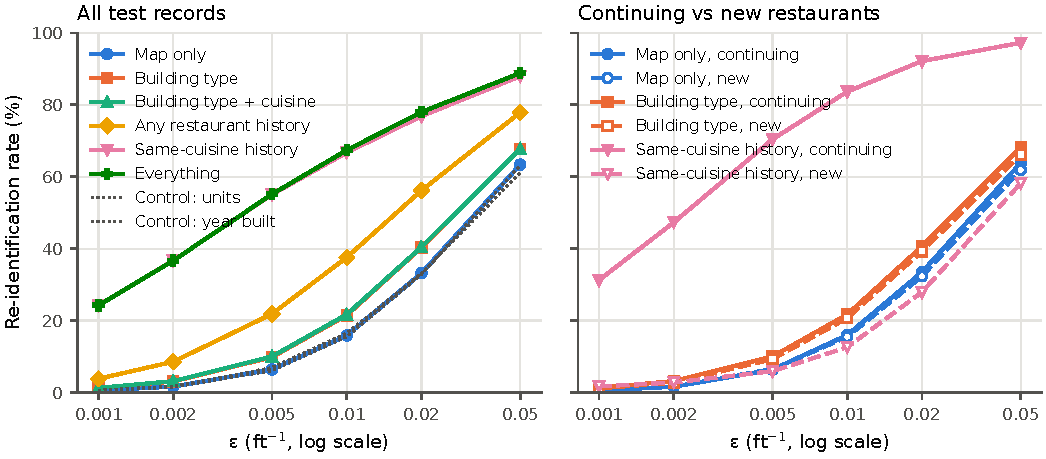
\includegraphics[width=\textwidth]{fig_single_query.pdf}
    \caption{Single-query re-identification rate vs $\varepsilon$ ($n = 45{,}052$ test visits). The left panel shows all priors, with 95\% Wilson intervals as shaded bands and dotted lines for the two negative controls. The right panel shows the map-only, building-type and same-cuisine history priors separately for restaurants present in the training data (continuing, solid) and new restaurants (dashed).}
    \label{fig:single_query}
\end{figure}

\begin{figure}[H]
    \centering
    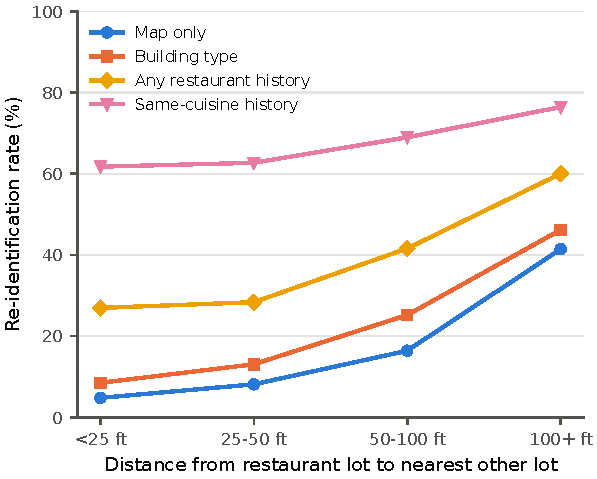
\includegraphics[width=0.55\textwidth]{fig_spacing.pdf}
    \caption{Re-identification rate at $\varepsilon = 0.01$ by distance from each restaurant's lot to the nearest other lot.}
    \label{fig:spacing}
\end{figure}

\subsection{Multi-record attack}

Releasing a linkable identifier (CAMIS) measurably degrades privacy, but the degradation is far less severe than the theoretical $n \cdot \varepsilon$ bound predicts. For map-only at $\varepsilon = 0.01$, restaurants with two inspections are re-identified 16.2\% of the time from a single record and 21.1\% when both are linked. For three inspections, 15.4\% and 27.4\%; for four, 13.6\% and 29.0\%. With same-cuisine history it is 66.7\% and 70.4\% for two inspections, 69.1\% and 75.8\% for three. Under map only, linked re-identification keeps rising with the number of inspections, but more slowly beyond three inspections. Under same-cuisine history, it changes little beyond three inspections (Figure~\ref{fig:multi_record}).

To test the composition bound, this paper compares the linked attack with a single release at the equivalent privacy level, comparing $n$ records released at $\varepsilon$ with one record released at $n\varepsilon$ for the same restaurants. Under map only at $\varepsilon = 0.01$, linking two records re-identifies 21.1\% of restaurants, against 33.7\% for a single release at $\varepsilon = 0.02$. For four records, 29.0\% against 54.2\% at $\varepsilon = 0.04$. The gap widens with $n$. The attacker combines linked records using their joint likelihood, so the shortfall does not come from a weak attack. It arises because each record receives independent noise, and averaging independent noise reduces the error only gradually (roughly with $\sqrt{n}$), whereas the composition bound allows privacy loss to grow linearly in $n$ as a worst case.

\begin{figure}[H]
    \centering
    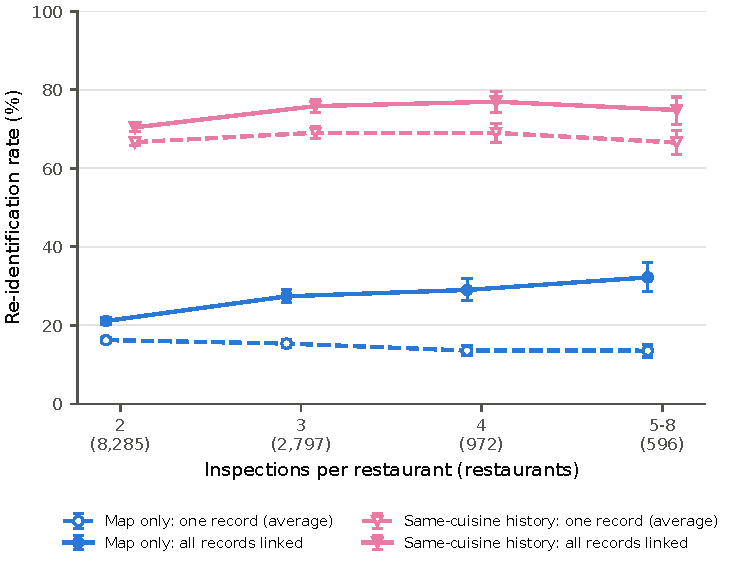
\includegraphics[width=0.7\textwidth]{fig_multi_record.pdf}
    \caption{Multi-record attack at $\varepsilon = 0.01$ for the map-only and same-cuisine history priors. For restaurants with exactly $n$ inspections (counts in parentheses, $n = 5$--$8$ pooled; the 15 restaurants with more than eight inspections are excluded), dashed lines show the average single-record re-identification rate across each restaurant's own inspections and solid lines show the rate when all inspections are linked. Error bars are 95\% intervals (Wilson for linked records, normal for the single-record average) for a single noise draw.}
    \label{fig:multi_record}
\end{figure}

\subsection{Posterior analysis}

The theoretical bound from Theorem 3.1 of Andr\'es et al.\ is satisfied in 100\% of tested records, and it is far from tight. Median empirical posterior-to-prior ratios range from 1.0 to 4.4 across configurations and $\varepsilon$ (1.4 to 4.4 for $\varepsilon \le 0.01$), and the largest ratio observed for any record is 558 (same-cuisine history, $\varepsilon = 0.001$). For each record, the bound $e^{\varepsilon D}$ is computed, where $D$ is the distance from the true lot to the farthest candidate in the search radius. Its median ranges from about 850 to 3,600 across settings, and the median ratio of a record's bound to its empirical posterior-to-prior ratio ranges from about 220 to 1,750. The bound therefore sits two to three orders of magnitude above what the attacker actually achieves.

Median attacker confidence in the true lot, $P(\text{true} \mid z)$, is 0.03\% at $\varepsilon = 0.001$ and about 2.6\% at $\varepsilon = 0.01$ (map only). At $\varepsilon \le 0.005$, fewer than 1.4\% of records have $P(\text{true} \mid z) > 0.5$ under the map-only and building-attribute priors, but up to 41.9\% do under same-cuisine history. Across all priors, this share is 2.7--59.8\% at $\varepsilon = 0.01$ and 49.2--87.0\% at $\varepsilon = 0.05$, the weakest privacy setting tested. Without restaurant history, then, the attacker's confidence in the true lot stays low in absolute terms at $\varepsilon \le 0.01$, even though median posterior-to-prior ratios of up to 4.4 mean that it rises by that factor.


\subsection{Utility loss}

Utility loss falls steadily as $\varepsilon$ increases (Figure~\ref{fig:utility}). Mean cuisine composition TVD falls from 0.45 at $\varepsilon = 0.001$ to 0.15 at $\varepsilon = 0.01$ (median 0.12, so roughly 12\% of a typical tract's cuisine distribution changes) and 0.02 at $\varepsilon = 0.05$. Inspection score RMSE falls from 4.55 points to 2.42 and 0.70 over the same range. Distortion arises because noise moves records across tract boundaries, so tract-level statistics mix records from neighboring tracts.

Privacy and utility therefore move in opposite directions (Figure~\ref{fig:tradeoff}). At $\varepsilon = 0.001$, location alone re-identifies 0.6\% of records, but nearly half of each tract's cuisine distribution changes. At $\varepsilon = 0.05$, distortion is negligible, but location alone re-identifies 63.4\% of records. At the intermediate value of $\varepsilon = 0.01$, mean TVD is 0.15 while the strongest attack still re-identifies 67.4\% of records.

\begin{figure}[H]
    \centering
    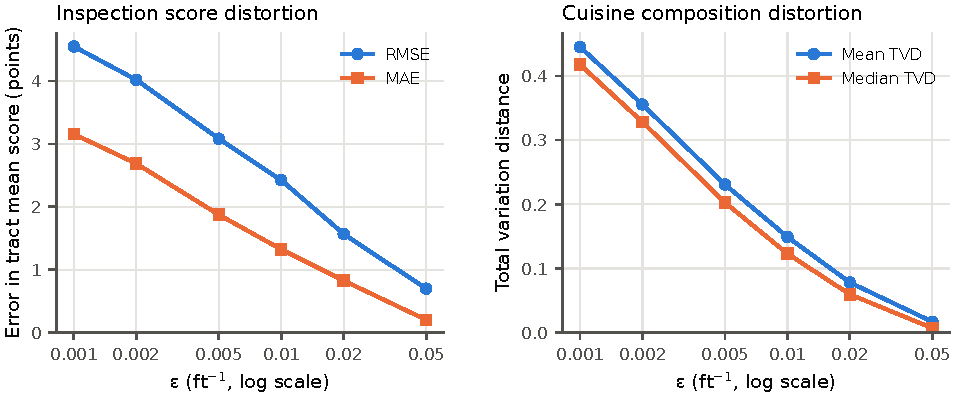
\includegraphics[width=\textwidth]{fig_utility.pdf}
    \caption{Utility loss vs $\varepsilon$, computed over 2020 Census tracts with restaurants both before and after noise, weighted by number of records. The left panel shows the error in tract mean inspection score (RMSE and MAE), and the right panel shows the total variation distance between true and noisy tract cuisine distributions (mean and median across tracts).}
    \label{fig:utility}
\end{figure}

\begin{figure}[H]
    \centering
    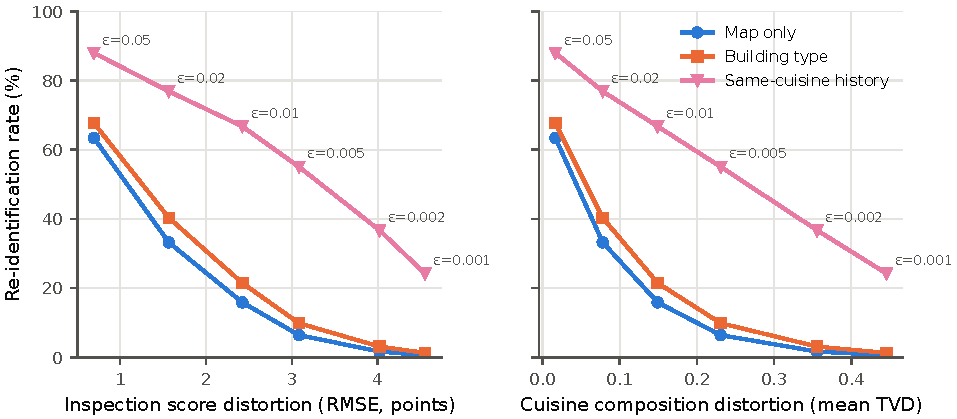
\includegraphics[width=\textwidth]{fig_tradeoff.pdf}
    \caption{Privacy-utility tradeoff. Re-identification rate against utility distortion for the map-only, building-type and same-cuisine history attacks; each point is one $\varepsilon$ (labeled on the same-cuisine history series).}
    \label{fig:tradeoff}
\end{figure}

\section{Discussion}\label{sec:discussion}

The central finding of this study is that the protection provided by the mechanism is systematically non-uniform. A record's exposure depends on how close its nearest similar lot is, and the priors available to the attacker determine which lots look similar. These record-level differences accumulate into differences between larger areas. Under the map-only prior, Staten Island and the Bronx are the least protected boroughs and Brooklyn the most protected at every $\varepsilon$ from 0.002 upward (Figure~\ref{fig:borough}). Under the history priors, the ranking changes and Manhattan becomes the most protected. This pattern follows from what counts as similar. Lots in general are most tightly packed in Brooklyn, while Manhattan restaurants are surrounded by lots of the same kind. Manhattan's high concentration of restaurants likely provides more same-cuisine look-alikes as well. This mechanism is not specific to restaurants. In any release under geo-indistinguishability, a record is exposed when no similar record lies within reach of the noise, with the released attributes determining which records count as similar and $\varepsilon$ determining the reach.

\begin{figure}[H]
    \centering
    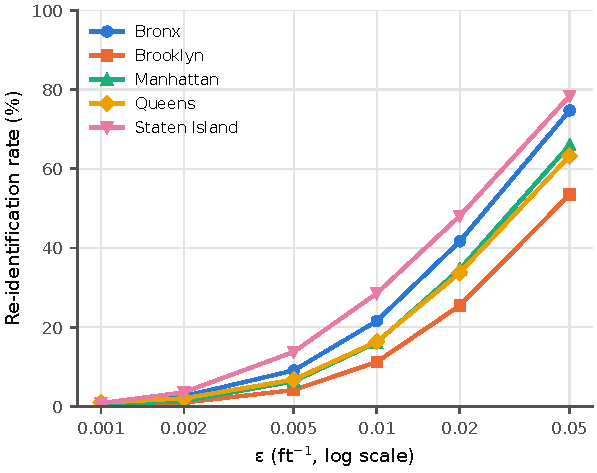
\includegraphics[width=0.6\textwidth]{fig_borough.pdf}
    \caption{Map-only re-identification rate vs $\varepsilon$ by borough.}
    \label{fig:borough}
\end{figure}

The comparison between Manhattan and Brooklyn also shows that the relevant notion of density is not always the intuitive one. Manhattan has about 3.6 times Brooklyn's built floor area per square mile but fewer than half as many lots per square mile, because its buildings are larger and sit on bigger lots. In this case, what protects a record against a location-only attacker is lot spacing, not floor-area density, so Brooklyn rather than Manhattan is the most protected borough in that setting.

Utility loss also differs by area. Manhattan loses the least utility, while the Bronx and Brooklyn lose the most. Part of this difference reflects how similar each tract is to its neighbors, since a record pushed into an adjacent tract distorts little when the two tracts have similar cuisine mixes, and part reflects the number of records per tract. These two characteristics account for roughly 36\% and 23\% of the gap between boroughs, respectively. Unfortunately, the drivers of utility loss are less clear-cut than those of re-identification, and much of the variation remains unexplained.

These differences suggest that a data publisher could tune the privacy parameter by region based on the more realistic case rather than the worst case (which treats every region the same). In this release, Staten Island and the Bronx would warrant a lower $\varepsilon$ than Brooklyn and Manhattan. Conversely, Brooklyn, which is well protected against a location-only attacker but is among the boroughs that lose the most utility, could tolerate a higher $\varepsilon$, avoiding unnecessary distortion. This mirrors guidance in the geographic masking literature that displacement should be inversely proportional to local population density (Zandbergen, 2014), but these results add a caveat. The density that matters is the density of records that look alike to the attacker, not of people or buildings (as seen in the case of Brooklyn and Manhattan). Understanding how neighbor similarity interacts with the priors an attacker could hold may help publishers identify vulnerable groupings beyond standard geographic units such as boroughs, and the same analysis can be repeated for other geocoded releases.

A second takeaway is that earlier releases shape how well a later release is protected. The most informative priors in this study were built from earlier, unprotected releases that linked restaurants to exact lots. These priors were highly effective for continuing restaurants but actually misleading for new ones. How vulnerable a release is therefore also depends on how much of it overlaps with earlier data. This dataset has a low turnover, making it more vulnerable. Areas with high turnover, such as those being redeveloped, may correspondingly be better protected. More generally, any dataset that moves from exact to noisy coordinates inherits the exposure of its earlier releases. A publisher can anticipate the scale of this by checking which released entities also appear in earlier, unprotected releases.

Linkable identifiers add a smaller cost. Releasing a restaurant identifier that links repeated inspections raises re-identification only modestly, and here linkage lets the public track restaurants with repeated violations (one of the main uses of inspection data). So, keeping it seems justified. Because independent noise averages out only slowly, the cost of linkage is modest in general, but it grows with the number of records per entity, so publishers of datasets with many records per entity should weigh it more carefully.

Finally, this analysis provides realized risk under realistic attackers alongside the worst-case bounds provided by the mechanism. The bounds hold for every record but greatly overstate the realized privacy loss. A publisher who chooses $\varepsilon$ from the bounds alone will therefore add more noise, and lose more utility, than the realized risk requires, while one who ignores what attackers already know may add too little. This is the gap between formal guarantees and realized risk at the center of the Census debate, and, as Ruggles and Van Riper (2022) argued for the Census Bureau's reconstruction experiment, measuring realized risk requires baselines that separate genuine information from chance, which the map-only prior and negative controls provide here. The privacy-utility curves (Figure~\ref{fig:tradeoff}) quantify the tradeoff that policymakers face. They also show that the tradeoff depends on both the utility metric chosen and the prior being evaluated, which makes the choice of these parameters an important part of any release decision.

\textbf{Limitations.} The attribute-based priors were chosen by exploring the available PLUTO attributes, such as the distribution of land use by cuisine (Figure~\ref{fig:prior_heatmap}), rather than derived from a model of attacker behavior, while the history priors follow from the threat model. Together, the priors do not exhaust what an attacker could know, so the reported rates are a lower bound on the risk from better-informed attackers; the negative controls guard against crediting gains to uninformative priors but do not address priors this study did not consider. The evaluation is also specific to New York City's dense urban environment. In suburban or rural settings, where similar records are farther apart, the same $\varepsilon$ would likely leave more records without look-alikes within reach of the noise. Results are based on a single noise draw per $\varepsilon$; the large sample keeps aggregate rates stable, but individual records would be exposed differently under another draw. The floor on zero shares ($10^{-10}$) in prior construction affects the balance between prior and spatial likelihood. Finally, candidate sets were limited to reduce computational cost (a restricted search radius, and an intersection requirement in multi-record attacks), so removing these restrictions could yield slightly higher attack success.

\textbf{Future work.} Natural extensions include spatially adaptive $\varepsilon$ calibrated to the local density of look-alike records; comparison with other location-protection mechanisms, such as deterministic rounding, the geographic masks used in health geography, and the exponential mechanism; posterior confidence ($P(\text{true} \mid z) > \text{threshold}$) as a stricter privacy metric; extension to non-Euclidean metric spaces ($d_X$-privacy; Chatzikokolakis et al., 2013); and a one-to-one bipartite matching attack enforcing the constraint that each lot can only be matched once.

\section*{References}

\noindent Andr\'es, M.~E., Bordenabe, N.~E., Chatzikokolakis, K., \& Palamidessi, C. (2013). Geo-indistinguishability: Differential privacy for location-based systems. \textit{Proceedings of the 2013 ACM SIGSAC Conference on Computer and Communications Security (CCS~'13)}, 901--914.

\noindent boyd, d., \& Sarathy, J. (2022). Differential perspectives: Epistemic disconnects surrounding the U.S. Census Bureau's use of differential privacy. \textit{Harvard Data Science Review}, Special Issue 2.

\noindent Brownstein, J.~S., Cassa, C.~A., \& Mandl, K.~D. (2006). No place to hide: Reverse identification of patients from published maps. \textit{New England Journal of Medicine}, 355(16), 1741--1742.

\noindent Chatzikokolakis, K., Andr\'es, M.~E., Bordenabe, N.~E., \& Palamidessi, C. (2013). Broadening the scope of differential privacy using metrics. \textit{Proceedings on Privacy Enhancing Technologies (PETS)}.

\noindent de Montjoye, Y.-A., Hidalgo, C.~A., Verleysen, M., \& Blondel, V.~D. (2013). Unique in the crowd: The privacy bounds of human mobility. \textit{Scientific Reports}, 3, 1376.

\noindent Dwork, C., McSherry, F., Nissim, K., \& Smith, A. (2006). Calibrating noise to sensitivity in private data analysis. \textit{Theory of Cryptography Conference (TCC)}.

\noindent Hotz, V.~J., Bollinger, C.~R., Komarova, T., Manski, C.~F., Moffitt, R.~A., Nekipelov, D., Sojourner, A., \& Spencer, B.~D. (2022). Balancing data privacy and usability in the federal statistical system. \textit{Proceedings of the National Academy of Sciences}, 119, e2104906119.

\noindent Kenny, C.~T., Kuriwaki, S., McCartan, C., Rosenman, E.~T.~R., Simko, T., \& Imai, K. (2021). The use of differential privacy for census data and its impact on redistricting: The case of the 2020 U.S. Census. \textit{Science Advances}, eabk3283.

\noindent Kenny, C.~T., Kuriwaki, S., McCartan, C., Rosenman, E.~T.~R., Simko, T., \& Imai, K. (2023). Comment: The essential role of policy evaluation for the 2020 Census disclosure avoidance system. \textit{Harvard Data Science Review}, Special Issue 2.

\noindent Kwan, M.-P., Casas, I., \& Schmitz, B.~C. (2004). Protection of geoprivacy and accuracy of spatial information: How effective are geographical masks? \textit{Cartographica}, 39(2), 15--28.

\noindent NYC Department of City Planning. (2026). \textit{Primary Land Use Tax Lot Output (PLUTO)}, version 26v2. NYC Open Data.

\noindent NYC Department of Health and Mental Hygiene. (2026). \textit{DOHMH New York City Restaurant Inspection Results}. NYC Open Data.

\noindent Reiter, J.~P. (2005). Estimating risks of identification disclosure in microdata. \textit{Journal of the American Statistical Association}, 100(472), 1103--1112.

\noindent Ruggles, S., Fitch, C., Magnuson, D., \& Schroeder, J. (2019). Differential privacy and census data: Implications for social and economic research. \textit{AEA Papers and Proceedings}, 109, 403--408.

\noindent Ruggles, S., \& Van Riper, D. (2022). The role of chance in the Census Bureau database reconstruction experiment. \textit{Population Research and Policy Review}, 41(3).

\noindent Sweeney, L. (2000). Simple demographics often identify people uniquely. \textit{Carnegie Mellon University, Data Privacy Working Paper 3}.

\noindent Sweeney, L. (2002). $k$-anonymity: A model for protecting privacy. \textit{International Journal of Uncertainty, Fuzziness and Knowledge-Based Systems}, 10(5), 557--570.

\noindent Zandbergen, P.~A. (2014). Ensuring confidentiality of geocoded health data: Assessing geographic masking strategies for individual-level data. \textit{Advances in Medicine}, 2014.

\end{document}
